\section{Analysis / Our approach} % (fold)
\label{sec:own_approach}

The \crowdre{} dataset is available in form of a MySQL database dump, but the tables can also be downloaded separated into several \textit{.csv} files\footnote{\url{https://crowdre.github.io/murukannaiah-smarthome-requirements-dataset/}, last visited 2020-01-15}. For our research, we were only interested in the pure requirement sentences (without any ratings, or user characterization added to the data). We could therefore reconstructed the sentences from the \textit{requirements.csv} file only, which is included in the downloaded data.

To have a benchmark for the approaches we want to use we need a labelling at the dataset that we can use to rate how good the topic modelling worked. At first we checked if we can use the tags as soft labelling for the requirements but unfortunately most of them are only matched once (Total tags: 2116, tags that only occur once: 1562). We also checked the amount of requirements represented by the most common tags. 

\begin{figure}[h]
  \centering
    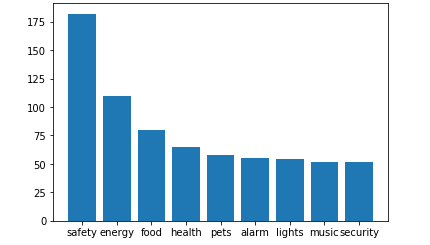
\includegraphics[width=\textwidth]{screenshots/tag_analysis.png}
    \caption{Tag occurence and coverage of the requirements}
    \label{fig:tag_analysis}
\end{figure}

In \autoref{fig:tag_analysis} it is obvious that the high amount of tags that only occur once lead to the fact that the relation between requirements is not working good. The variety of tags that may be assigned to the same topic is very high and the low coverage of requirements with the top 9 tags makes the tags not suitable for the soft labelling. So we checked the domains that were assigned to the requirements. The domains are separated into five groups: Health, Energy, Entertainment, Safety and Other. For the \grqq{}Other\grqq{} there are again user defined specific domains, but we focus on the five top level domains for our labelling.

\colorbox{yellow!30}{ToDo:} Give the approach a name as title!

\subsection{NLP Preprocessing Pipeline} % (fold)
\label{sub:own_pipeline}

\begin{figure}[ht]
  \caption{Our NLP Preprocessing Pipeline and an exemplaric requirement sentence.}
  \centering
    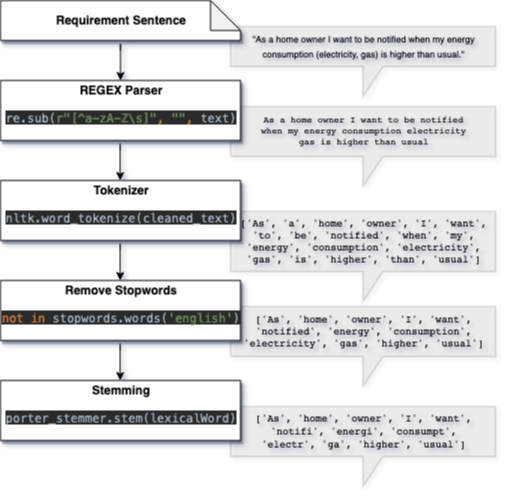
\includegraphics[width=\textwidth]{figures/NLP Pipeline.png}
    \label{fig:nlp_pipeline}
\end{figure}

As initially described in section \ref{sec:nlp} we preprocessed our requirement documents using an NLP pipeline as shown in figure \ref{fig:nlp_pipeline}. Implementing our solution in Python and following the common practice as suggested in \cite{ferrari_natural_2018}, we made use of the NLTK library\footnote{\url{https://www.nltk.org/}, last visited 2020-01-18} to perform the NLP techniques we needed for our analysis. As some of the requirements sentences contained special characters, some initial data cleansing was necessary, to remove these special characters (i.e. spaces, dots, apostrophes, slashes) as they would have otherwise been ranked in the later used bag of words. We used regular expressions as provided by the Python standard library in order to do so. For the tokenization, the stop-word-removal and the stemming we used the functions provided by the NLTK API.
% subsection preprocessing (end)

\subsection{LDA Approach} % (fold)
\label{sub:own_lda}
After we developed our pre-processing pipeline for the dataset and some basic analysis on the data we have we decided to use the LDA for a first topic modelling. The idea was to have another approach in the first step that we can use as intermediate result for the data and also to compare it to the result of the neural network to have some kind of benchmark or basis for a performance comparison.


For our LDA approach we used our preprocessed requirements. To apply an LDA to the data we need an array of arrays where each inner array represents a single requirement (so in this dimension it has 2966 entries). each word in the requirements needs to be replaces by a number that can be processed by the LDA. So we first applied a bag-of-words which calculates a relative weight for the single words. the next step is rating the words with the TF-IDF. After these steps we have a prepared matrix that contains the data that now can be processed by the LDA.

\begin{figure}[h]
  \begin{center}
    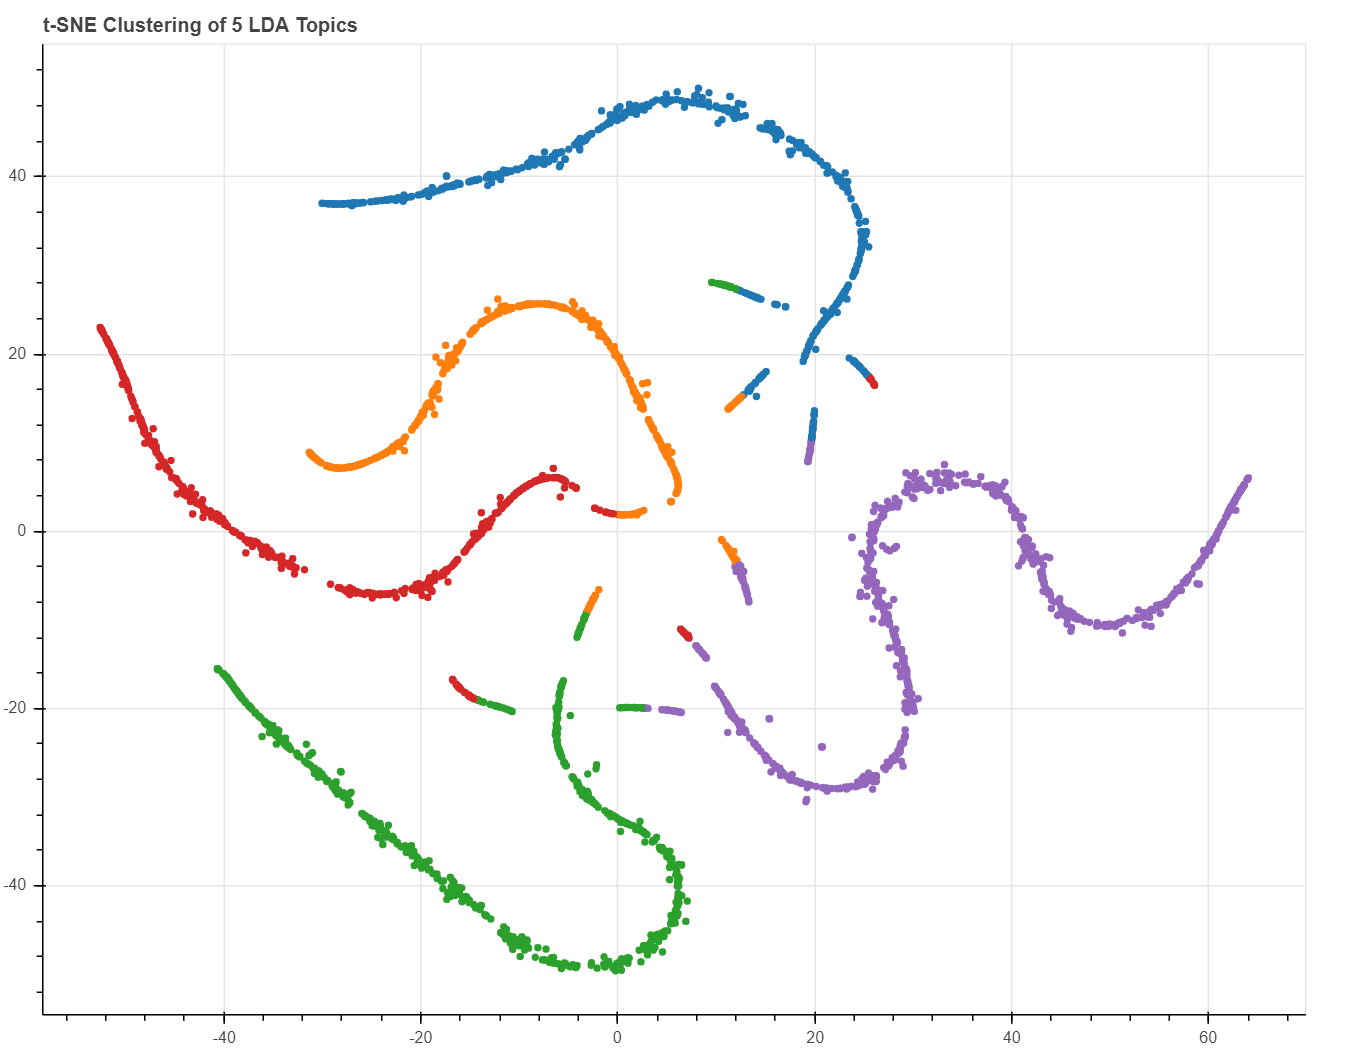
\includegraphics[width=\textwidth]{screenshots/lda-tf-idf.png}
    \caption{LDA Result with TF-IDF (plotted with t-SNE)}
    \label{fig:lda-tf-idf}
  \end{center}
\end{figure}

In \autoref{fig:lda-tf-idf} we can see the result of the LDA that is plotted using t-SNE. The colors represent the different topics that were generated.

\subsection{Neural Network} % (fold)
\label{sub:own_neuralnetwork}

\colorbox{yellow!30}{ToDo:} How does our approach with the Neural Network looks like?
